\documentclass[11pt]{article}

\usepackage[utf8]{inputenc}
\usepackage[T1]{fontenc}
\usepackage{textcomp}
\usepackage{helvet}
\usepackage[margin=1in]{geometry}
\usepackage{graphicx}
\usepackage{booktabs}
\usepackage{array}
\usepackage{tabularx}
\usepackage{amsmath,amssymb}
\usepackage{xcolor}
\usepackage{setspace}
\usepackage{caption}
\usepackage{url}
\usepackage[numbers,sort&compress]{natbib}
\usepackage{hyperref}
\hypersetup{colorlinks=true, linkcolor=navy, citecolor=navy, urlcolor=navy}

\definecolor{navy}{HTML}{0B2E4F}
\definecolor{gold}{HTML}{C99700}
\captionsetup{font=small, labelfont=bf, width=0.95\textwidth}
\setlength{\parskip}{4pt}
\renewcommand{\arraystretch}{1.15}

% Report numbers are generated from the frozen release so that the narrative
% and the figures use one consistent set of counts.
% Generated by technical_report/make_figures.py -- do not edit by hand.
% One macro per number the report quotes; rerun the script to refresh.
\newcommand{\nBasisGrams}{11}
\newcommand{\nBasisMixed}{18}
\newcommand{\nBasisPartsPerHundred}{447}
\newcommand{\nBasisUnspecified}{1}
\newcommand{\nBasisWeightPct}{124}
\newcommand{\nCiHiBlendEmbdescFifty}{+0.234}
\newcommand{\nCiHiCategories}{+0.189}
\newcommand{\nCiHiDescriptorsVisc}{+0.092}
\newcommand{\nCiHiEmbWeighted}{+0.254}
\newcommand{\nCiLoBlendEmbdescFifty}{-0.059}
\newcommand{\nCiLoCategories}{-0.115}
\newcommand{\nCiLoDescriptorsVisc}{-0.046}
\newcommand{\nCiLoEmbWeighted}{-0.074}
\newcommand{\nCorpusDocs}{2,925}
\newcommand{\nCsCompDocs}{161}
\newcommand{\nCsCompRows}{3,080}
\newcommand{\nCsCondDocs}{85}
\newcommand{\nCsCondRows}{1,992}
\newcommand{\nCsDocs}{183}
\newcommand{\nCsPopulation}{3,862}
\newcommand{\nCsRows}{3,961}
\newcommand{\nCureCatalystForms}{409}
\newcommand{\nCureInitiatorForms}{183}
\newcommand{\nCureUnnamedForms}{13}
\newcommand{\nDeltaBlendEmbdescFifty}{+0.088}
\newcommand{\nDeltaCategories}{+0.037}
\newcommand{\nDeltaDescriptorsVisc}{+0.023}
\newcommand{\nDeltaEmbWeighted}{+0.090}
\newcommand{\nDocMaxRows}{93}
\newcommand{\nDocMedianRows}{8}
\newcommand{\nEmbDims}{768}
\newcommand{\nEmbDistinct}{124}
\newcommand{\nEmbForms}{605}
\newcommand{\nEmbStrings}{945}
\newcommand{\nEmbZeroForms}{183}
\newcommand{\nGroupedBlendEmbdescFifty}{0.234}
\newcommand{\nGroupedCategories}{0.209}
\newcommand{\nGroupedConditions}{0.258}
\newcommand{\nGroupedDescriptorsVisc}{0.157}
\newcommand{\nGroupedEmbWeighted}{0.199}
\newcommand{\nGroupedXgbConditions}{0.145}
\newcommand{\nLadderRepeats}{30}
\newcommand{\nLofoBlendEmbdescFifty}{0.278}
\newcommand{\nLofoCategories}{0.228}
\newcommand{\nLofoConditions}{0.289}
\newcommand{\nLofoDescriptorsVisc}{0.213}
\newcommand{\nLofoEmbWeighted}{0.280}
\newcommand{\nLofoMaeBlendEmbdescFifty}{17.5}
\newcommand{\nLofoMaeCategories}{17.5}
\newcommand{\nLofoMaeConditions}{17.5}
\newcommand{\nLofoMaeDescriptorsVisc}{18.1}
\newcommand{\nLofoMaeEmbWeighted}{17.2}
\newcommand{\nLofoXgbConditions}{0.190}
\newcommand{\nPropDocs}{1,930}
\newcommand{\nProtocolDistinct}{60}
\newcommand{\nProtocolSeventyHOneFifty}{28}
\newcommand{\nProtocolTwentyTwoHOneSevenFive}{124}
\newcommand{\nRandomBlendEmbdescFifty}{0.669}
\newcommand{\nRandomCategories}{0.737}
\newcommand{\nRandomConditions}{0.401}
\newcommand{\nRandomDescriptorsVisc}{0.548}
\newcommand{\nRandomEmbWeighted}{0.690}
\newcommand{\nReactAlkenyl}{153}
\newcommand{\nReactNonReactive}{7}
\newcommand{\nReactSih}{1}
\newcommand{\nReactSilanol}{30}
\newcommand{\nReactUnknownReactivity}{42}
\newcommand{\nRelDistinctIngredients}{945}
\newcommand{\nRelDocs}{67}
\newcommand{\nRelForms}{605}
\newcommand{\nRelGroups}{66}
\newcommand{\nRelIQRhi}{51}
\newcommand{\nRelIQRlo}{13}
\newcommand{\nRelIngredientRows}{4,898}
\newcommand{\nRelJournals}{2}
\newcommand{\nRelMean}{33.7}
\newcommand{\nRelMedian}{25}
\newcommand{\nRelPatents}{65}
\newcommand{\nRelRows}{1,054}
\newcommand{\nRelYearMax}{2026}
\newcommand{\nRelYearMin}{1974}
\newcommand{\nReleaseComponentRows}{4,898}
\newcommand{\nReleaseDistinctStrings}{945}
\newcommand{\nResAllPct}{50}
\newcommand{\nResDeflectionPct}{81}
\newcommand{\nResIngredientsPct}{80}
\newcommand{\nResTempPct}{72}
\newcommand{\nResTimePct}{72}
\newcommand{\nResValuePct}{92}
\newcommand{\nRoleBasePolymerPct}{98}
\newcommand{\nRoleCatalystPct}{68}
\newcommand{\nRoleCrosslinkerPct}{73}
\newcommand{\nRoleInitiatorPct}{30}
\newcommand{\nRoleReinforcingFillerPct}{72}
\newcommand{\nRowAllPct}{7}
\newcommand{\nRowDeflectionPct}{14}
\newcommand{\nRowIngredientsPct}{80}
\newcommand{\nRowTempPct}{46}
\newcommand{\nRowTimePct}{50}
\newcommand{\nRowValuePct}{92}
\newcommand{\nSpellTopCount}{221}
\newcommand{\nSpellTopRole}{base polymer}
\newcommand{\nSpgBlendEmbdescFifty}{0.21}
\newcommand{\nSpgCategories}{0.22}
\newcommand{\nSpgDescriptorsVisc}{0.10}
\newcommand{\nSpgEmbWeighted}{0.23}
\newcommand{\nSpgMax}{0.23}
\newcommand{\nSpgMin}{0.10}
\newcommand{\nStatedDeflection}{100}
\newcommand{\nStatedMedium}{100}
\newcommand{\nStatedSpecimenDiameter}{51}
\newcommand{\nStatedSpecimenShape}{60}
\newcommand{\nStatedSpecimenThickness}{51}
\newcommand{\nStatedTemperature}{100}
\newcommand{\nStatedTestStandard}{49}
\newcommand{\nStatedTime}{100}
\newcommand{\nUmapBasePolymers}{233}
\newcommand{\nUmapDims}{768}
\newcommand{\nUmapDistinct}{440}
\newcommand{\nUmapForms}{605}
\newcommand{\nUmapMissing}{0}
\newcommand{\nUmapStrings}{945}
\newcommand{\nUmapTopDocShare}{36}


\newcommand{\release}{cs\_v14}
\newcommand{\degC}{\,\textdegree C}

\title{\vspace{-1.5em}
  {\large TECHNICAL PROGRESS REPORT}\\[0.6em]
  {\LARGE\bfseries Source-Linked Compression-Set Data for Silicone Formulations}\\[0.4em]}
\author{Bryan V.\ Piguave \and Brett M.\ Savoie\\[0.4em]
  \normalsize Department of Chemical and Biomolecular Engineering, University of Notre Dame\\
  \normalsize Notre Dame, IN 46556, USA\\[0.6em]}
\date{September 17, 2026}

\begin{document}
\maketitle

% ---------------------------------------------------------------------------
\section*{Executive summary}
% ---------------------------------------------------------------------------
This report summarizes the work completed to assemble a source-linked record
of silicone formulations and compression-set measurements from patents and
journal articles. The practical question is whether a documented formulation
and its test conditions can support useful guidance for seal design without
requiring a new compression-set experiment for every candidate.

The main result is a funnel. We began with \nCorpusDocs{} downloaded documents.
\nPropDocs{} contained at least one extracted property, \nCsDocs{} reported a
compression-set value, and only \nCsCondDocs{} provided a value together with
a composition and the three essential test conditions: temperature, time, and
deflection. After source checking and curation, the current release contains
\nRelRows{} measurements over \nRelForms{} formulations from \nRelDocs{}
documents. The decrease is not a failure of the project; it identifies the
amount of the published record that is sufficiently described to support
quantitative comparison.

The release also distinguishes the material classes that are important for
interpreting the data. A formulation is counted as a composite when it
contains a dispersed filler role, and as a foam when it contains a blowing
agent role. There are \nCompositeForms{} composite formulations and
\nFoamForms{} foam formulations. \nCompositeFoamForms{} formulations belong to
both groups; the remaining formulations are \nCompositeOnlyForms{} composite
only, \nFoamOnlyForms{} foam only, and \nNeitherForms{} neither.

The work produced a reliable baseline and a clear limitation. Test conditions
alone give a leave-one-family-out $R^2$ of \nLofoConditions{} with a mean
absolute error of \nLofoMaeConditions{} percentage points. The chemistry
representations examined so far do not produce a statistically separable
improvement when entire source families are held out. This does not mean that
chemistry is unimportant. It means that the present record is still too small,
too unevenly described, and too concentrated in a limited number of source
families to establish a transferable chemistry effect.

% ===========================================================================
\section{What are the major goals of the project?}
% ===========================================================================
Compression set is a useful engineering property because it measures how much
of an imposed deformation remains after an elastomer has been held under load
for a specified time and temperature \citep{astmd395}. It is directly related
to the long-term performance of seals, but it is also strongly dependent on
the test protocol. A value measured after 22~h at 175\degC{} is not directly
interchangeable with a value measured after 70~h at 150\degC{}.

The first goal is therefore to gather measurements together with the
conditions that make them interpretable. The second is to preserve the
chemistry of the formulation: base polymer, crosslinker, catalyst or
initiator, fillers, additives, and any blowing agent. Silicone elastomers are
not single-molecule materials. Their behavior depends on the network created
by the cure chemistry, the interaction with fillers, and the processing and
aging history \citep{mazurek2019silicone,yue2013tensile,patel2004stress}.

The third goal is to determine what can reasonably be learned from the
published record. Polymer formulations are difficult to model because the
design space is large while much of the practical knowledge is recorded in
qualitative descriptions, patents, and tables with inconsistent terminology
\citep{audus2017polymer,butler2018machine,ramprasad2017machine}. The project
therefore asks two separate questions: what information can be recovered and
checked, and how much predictive value does the recovered chemistry add beyond
the test conditions themselves?

% ===========================================================================
\section{What was accomplished under these goals?}
% ===========================================================================
The project established a complete path from a broad literature record to a
curated set of comparable measurements. Documents were collected from patents
and journal literature, screened for silicone materials and quantitative
compression-set results, and read in the context of the surrounding
formulation and testing descriptions. Duplicate source families were treated
as one scientific source so that repeated publication of the same work did
not create artificial evidence.

The result is summarized in Figure~\ref{fig:problem}. The top panel makes the
funnel explicit: each additional requirement removes documents that do not
provide enough information for a defensible comparison. The lower-right panel
records the material classes in the final release. These classes overlap by
design, because a filled silicone foam is both a composite and a foam.

\begin{figure}[t]
  \centering
  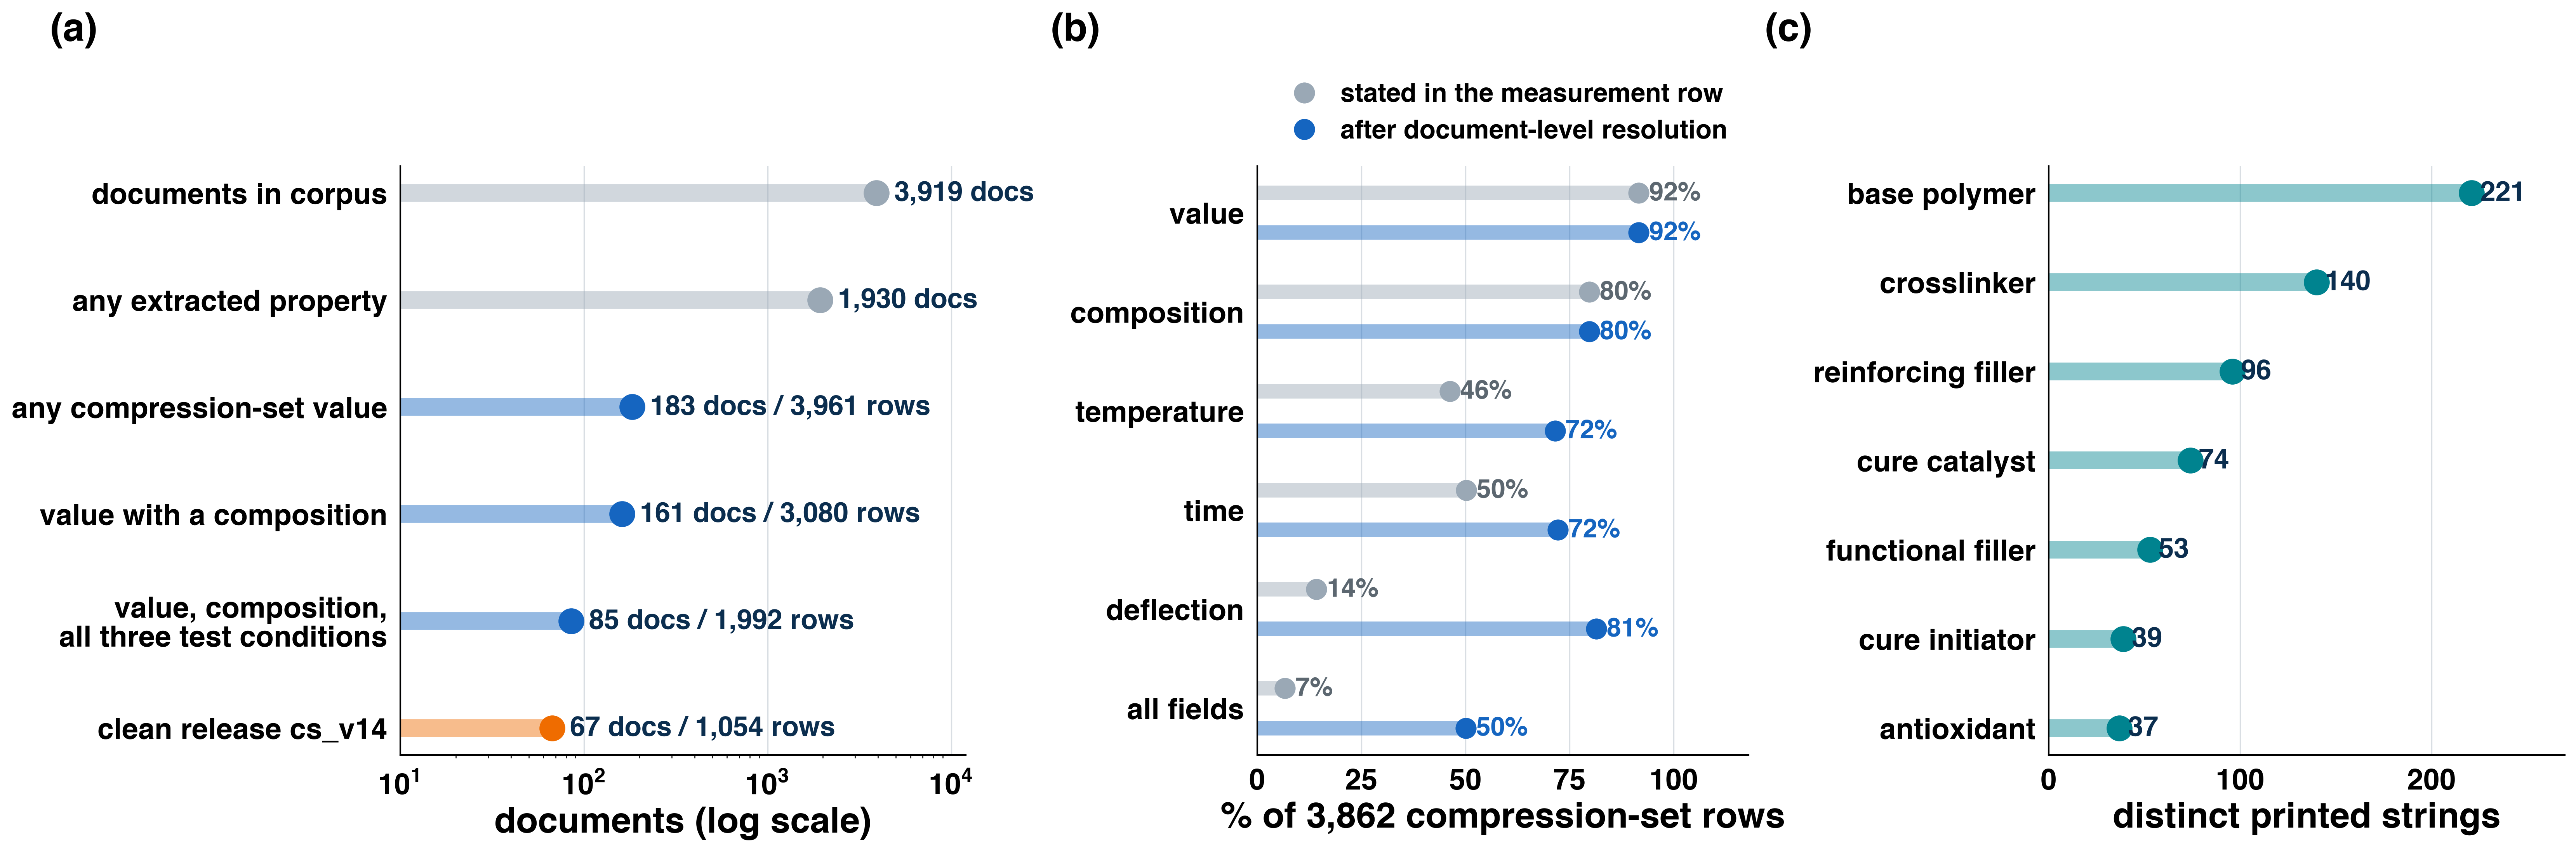
\includegraphics[width=\linewidth]{figures/problem_qualitative_record_vs_quantitative_compression_set_data.png}
  \caption{\textbf{The record narrows from documents to usable measurements.}
  (a) Documents remaining as composition, test protocol, and release-quality
  requirements are applied; row counts are shown where the stage is defined on
  measurements. (b) Information stated in the measurement row itself compared
  with information recovered from the document as a whole. (c) Formulations
  classified as composite, foam, both, or neither. Composite means a
  dispersed-filler role; foam means a blowing-agent role.}
  \label{fig:problem}
\end{figure}

\subsection{Major Activities}
The work had four connected activities. First, the source record was expanded
without requiring the property to appear in a title or abstract. This was
important because many patents present compression-set values only in example
tables. Second, formulations were read as recipes rather than as isolated
chemical names. Trade names, component labels, filler descriptions, cure
systems, and amount conventions were retained when they were part of the
source's description.

Third, test conditions were connected to the measurements to which they
belong. Temperature, time, deflection, medium, specimen geometry, and stated
test standard were kept separate because each can change how a compression-set
value should be interpreted. When a source stated conditions in a methods
paragraph rather than beside the result, the conditions were connected back to
the relevant measurements only when the source supported that connection.

Fourth, the resulting records were checked against the source pages. A
stratified audit found the released compression-set value correct in 96.8\% of
checkable cases, with a Wilson 95\% interval of 94.7--98.1\%. Temperature and
deflection were correct in every checked case. The audit also identified
specific table-reading failures and source-family duplicates that would have
been difficult to detect from numerical consistency alone.

\subsection{Specific Objectives}
\textbf{Objective 1 -- Build a quantitative source record.} The project
converted a dispersed set of patents and articles into a collection in which
each measurement remains connected to its source document, formulation, and
test description.

\textbf{Objective 2 -- Distinguish material classes.} The project now reports
which released formulations contain dispersed fillers and which contain
blowing agents. This makes the composite and foam populations visible instead
of combining them into one undifferentiated silicone category.

\textbf{Objective 3 -- Establish a defensible predictive baseline.} The
project compared condition-based prediction with several broad descriptions
of chemistry while keeping source families separate during evaluation. The
purpose was to identify what the current evidence supports, not to maximize a
single score by mixing related examples between training and testing.

% ===========================================================================
\section{Significant Results}
% ===========================================================================
\subsection{The document funnel identifies the quantitative core}
The funnel begins with \nCorpusDocs{} downloaded documents and ends with
\nRelDocs{} source documents in the current release. In between, the record
passes through \nPropDocs{} documents with any extracted property, \nCsDocs{}
documents with a compression-set value, \nCsCompDocs{} documents with a
stated composition, and \nCsCondDocs{} documents with a complete test
protocol. The corresponding compression-set row counts are \nCsRows{} for
the broad property population, \nCsCompRows{} with a composition, and
\nCsCondRows{} with all three conditions.

This sequence is the most important result for planning future work. A large
number of documents does not automatically create a large modeling dataset.
The limiting resource is the number of source families that report a complete
recipe, a measured value, and enough test information for comparison. The
funnel shows exactly where additional reading and curation can increase the
usable population.

\subsection{The release separates composites and foams}
The material classification is based on the ingredient roles supported by the
source. Composite means at least one reinforcing, functional, extending, or
lightweight filler. Foam means a blowing agent. The four categories below
partition the 605 released formulations, while the aggregate composite and
foam populations overlap.

\begin{table}[h]
\centering\small
\caption{Operational material classes in release \release. The composite and
foam labels can overlap; the four rows partition the formulations.}
\begin{tabular}{@{}lrr@{}}
\toprule
Formulation class & Formulations & Compression-set measurements \\
\midrule
Composite only & \nCompositeOnlyForms{} & \nCompositeOnlyRows{} \\
Composite and foam & \nCompositeFoamForms{} & \nCompositeFoamRows{} \\
Foam only & \nFoamOnlyForms{} & \nFoamOnlyRows{} \\
Neither composite nor foam & \nNeitherForms{} & \nNeitherRows{} \\
\midrule
Total & \nRelForms{} & \nRelRows{} \\
\bottomrule
\end{tabular}
\end{table}

In aggregate, \nCompositeForms{} formulations from \nCompositeDocs{} documents
are composites and \nFoamForms{} formulations from \nFoamDocs{} documents are
foams. The overlap is substantive rather than an accounting error: the
\nCompositeFoamForms{} formulations in both classes contribute to both totals.
This distinction should be carried into future comparisons because foam
structure, filler content, and cure conditions can affect compression set in
different ways.

\subsection{The current release is broad but uneven}
The current release \release{} contains \nRelRows{} measurements over
\nRelForms{} formulations from \nRelDocs{} documents, including \nRelPatents{}
patents and \nRelJournals{} journal articles published between \nRelYearMin{}
and \nRelYearMax{}. The median compression set is \nRelMedian\% and the
interquartile range is \nRelIQRlo--\nRelIQRhi\%. The sources use several
amount conventions and describe cure systems, fillers, and test geometries
with different levels of detail.

Figure~\ref{fig:dataset} summarizes this variation. The measurements are
unevenly distributed across source documents, and the test conditions cluster
around common industrial protocols while extending to other temperatures and
times. This unevenness is why the report emphasizes source families and
document-level comparison rather than treating every row as an independent
piece of evidence.

\begin{figure}[t]
  \centering
  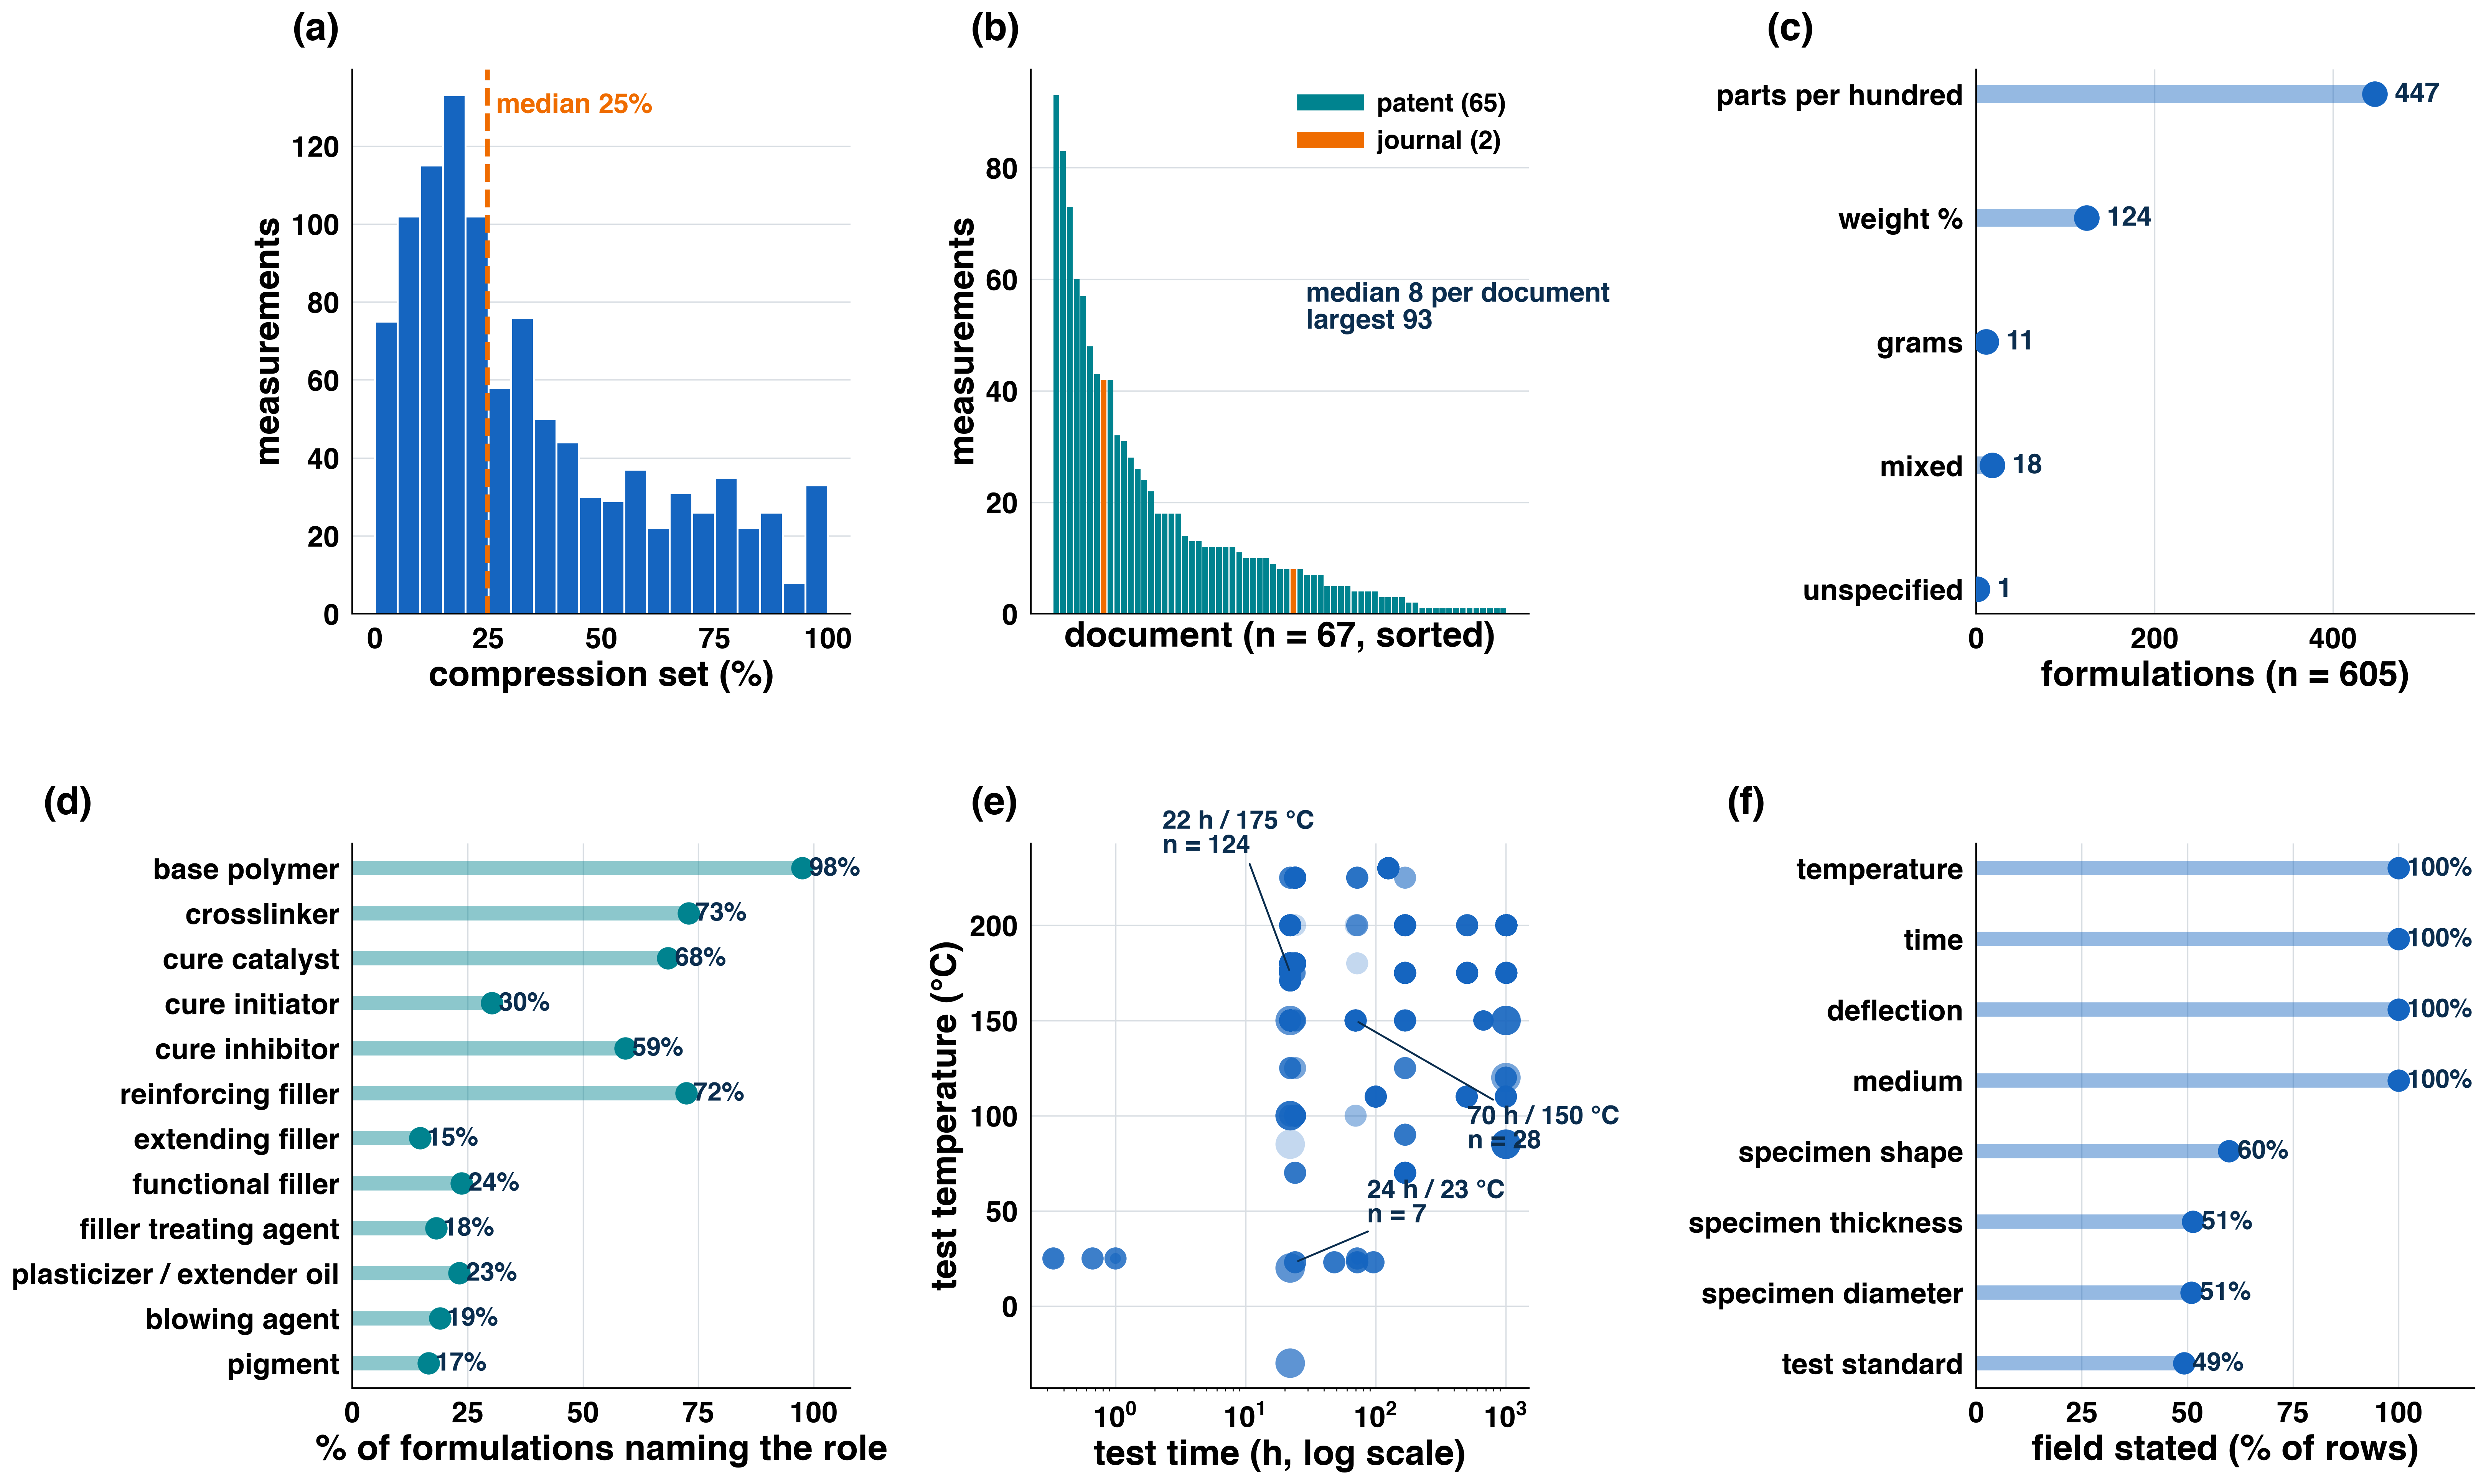
\includegraphics[width=\linewidth]{figures/release_cs_v14_target_sources_amount_basis_roles_protocols_and_field_coverage.png}
  \caption{\textbf{What the current release contains.} The release includes
  measurements spanning a wide range of compression-set values, source
  documents, formulation amount conventions, ingredient roles, and test
  protocols. Empty fields are retained as evidence that the source was silent;
  they are not silently filled by an assumed value.}
  \label{fig:dataset}
\end{figure}

\subsection{A conditions-only baseline is presently the defensible result}
The first predictive comparison used the test conditions as the common basis
for every formulation. Additional chemistry descriptions were then tested to
ask whether they improved transfer to source families that had not been used
to fit the prediction. Conditions alone reached a leave-one-family-out
$R^2$ of \nLofoConditions{} with a mean absolute error of
\nLofoMaeConditions{} percentage points.

Adding stated viscosity, ingredient descriptions, combined descriptors, or
ingredient categories changed the leave-one-family-out score by small amounts
whose uncertainty intervals included zero. The best chemistry representation
reached \nLofoEmbWeighted{}, but the current corpus cannot establish that this
is better than the conditions-only baseline. Random-row evaluation gives a
substantially higher diagnostic score, including \nRandomCategories{} for
ingredient categories, because related examples from the same document remain
on both sides of the comparison.

Figure~\ref{fig:ladder} presents this result as a model ladder. The main
conclusion is a statement about evidence: the present release supports a
useful condition-based baseline, but it does not yet support a claim that the
available chemistry descriptions improve prediction for unseen source
families. A larger and more balanced set of complete source families, or a
trusted validation set, is needed to answer that question.

\begin{figure}[t]
  \centering
  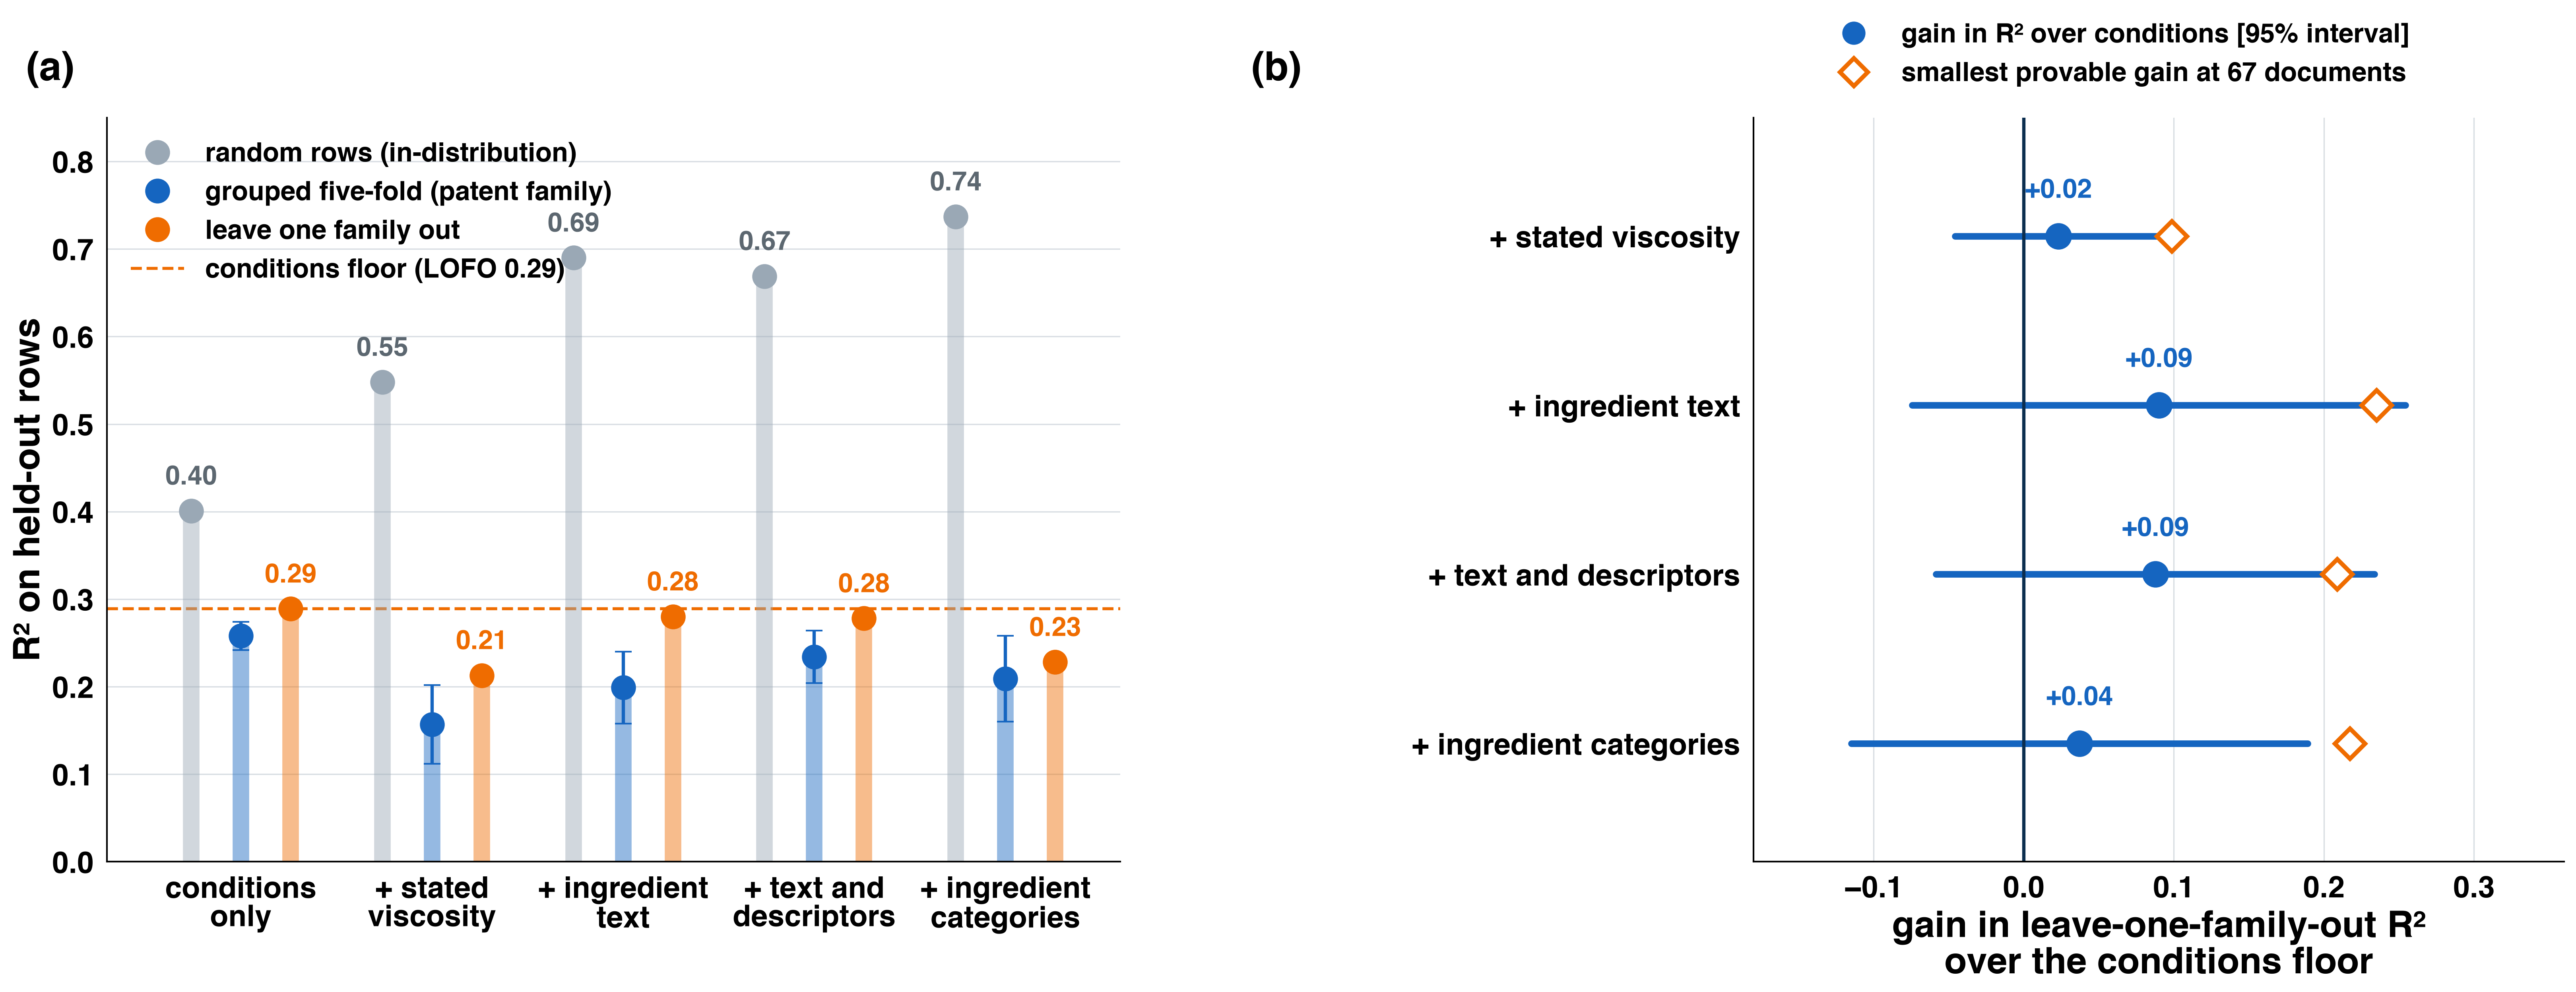
\includegraphics[width=\linewidth]{figures/ladder_conditions_floor_vs_chemistry_arms_grouped_random_and_paired_gain.png}
  \caption{\textbf{The predictive baseline and the chemistry question.} The
  conditions-only baseline is compared with several broad chemistry
  descriptions under familiar-document and unseen-family evaluations. The
  chemistry gains remain within the uncertainty supported by the current
  number of source families.}
  \label{fig:ladder}
\end{figure}

% ===========================================================================
\section{Lessons from verification}
% ===========================================================================
Several verification cases changed the way the record is interpreted. A
correct numerical value can still be attached to the wrong formulation when
two members of a patent family present different tables. A plausible chemical
name can still be wrong when a source uses a similar-looking end group. A
table can appear complete while a shifted column has assigned an amount or a
test condition to the neighboring row. These cases show why numerical
agreement, chemical plausibility, and direct source checking are all needed.

The most consequential lesson is that source context matters more than the
title of a document. Some documents that appear general from their title
contain the most useful aging data, while some documents that mention silicone
do not describe a silicone matrix and should not be included. The funnel and
the audit are therefore complementary: the funnel shows how many documents
remain, while the audit tests whether the surviving values still mean what the
source reported.

% ===========================================================================
\section{Companion benchmark and broader value}
% ===========================================================================
The table-reading work was also tested on a 1968 reference volume containing
tabulated organosilicon properties. That setting offered a fixed ground truth
against which names, structures, values, and pressures could be checked. The
verified benchmark contains 509 measurements over 436 structures from 159
references. The benchmark was useful because it separated errors in reading a
table from uncertainty in interpreting a modern patent formulation.

The broader contribution is a change in the unit of analysis. Silicone
formulation development is often discussed in terms of individual ingredients
or isolated property values. The present record connects the source document,
the complete formulation, the material class, and the test protocol. That
connection makes it possible to ask which evidence is genuinely comparable
and which apparent trend is only a consequence of how a document was written.

% ===========================================================================
\section{How have the results been disseminated?}
% ===========================================================================
The results are being organized as a technical report, a frozen research
release, source-linked records for the collaborating group, and a documented
set of figures that communicate both the size of the record and its limits.
The funnel is intended to make acquisition priorities visible to collaborators:
new documents are valuable when they add complete formulations and complete
test conditions, not merely when they increase the number of downloaded
papers.

The report also provides a common language for discussing material classes.
Future meetings can distinguish filled silicone composites, silicone foams,
and formulations that belong to both categories instead of comparing all of
them as one population.

% ===========================================================================
\section{What do you plan to do next to accomplish the goals?}
% ===========================================================================
The next stage has three priorities. First, confirmed errors from the audit
will be corrected and additional source families will be added through the
same source-linked process. Second, the composite and foam labels will be
reviewed alongside cure system and base-polymer information so that the
material classes can be compared without conflating structure and chemistry.
Third, the predictive baseline will be reevaluated after the record is
expanded and after collaborators provide a small validation set with trusted
formulations and test conditions.

Two inputs from collaborators would have immediate value. A set of
formulations that Los Alamos trusts, with or without measured values, would
provide a fixed reference for evaluating extraction and representation choices.
Also needed is a statement of what prediction error would change a design
decision at a named test protocol. That engineering threshold would determine
whether the next effort should focus on more source families, more complete
chemistry descriptions, or targeted measurements of composites and foams.

% ===========================================================================
\section{Information retained in the research release}
% ===========================================================================
Each released measurement remains connected to its source document and to the
formulation from which it was reported. The retained information includes the
ingredient descriptions and roles, amounts and amount conventions, measured
compression set, test temperature, time, deflection, and any stated medium,
specimen geometry, or post-cure history. Missing information is left visible
as missing so that future users can distinguish a source that did not report a
quantity from a formulation that did not contain or require it.

The current release is a snapshot of the evidence available at this stage of
the project. Its value is not only the number of rows; it is the traceability
that allows a future correction, new material class, or new test condition to
be connected back to the page on which the original claim was made.

\bibliographystyle{unsrtnat}
\bibliography{references}

\end{document}
